% Compile from docs/research with latexmk -xelatex -no-shell-escape out-accelerate.tex
\documentclass[11pt,letterpaper]{article}
\usepackage{lmodern}
\usepackage{fontspec}
\IfFontExistsTF{TeX Gyre Pagella}{\setmainfont{TeX Gyre Pagella}}{
 \IfFileExists{/usr/share/fonts/opentype/urw-base35/P052-Roman.otf}{
  \setmainfont[Path=/usr/share/fonts/opentype/urw-base35/,UprightFont=*-Roman.otf,BoldFont=*-Bold.otf,ItalicFont=*-Italic.otf,BoldItalicFont=*-BoldItalic.otf]{P052}
 }{\setmainfont{Latin Modern Roman}}}
\IfFontExistsTF{TeX Gyre Heros}{\setsansfont{TeX Gyre Heros}}{
 \IfFileExists{/usr/share/fonts/opentype/urw-base35/NimbusSans-Regular.otf}{
  \setsansfont[Path=/usr/share/fonts/opentype/urw-base35/,UprightFont=*-Regular.otf,BoldFont=*-Bold.otf,ItalicFont=*-Italic.otf,BoldItalicFont=*-BoldItalic.otf]{NimbusSans}
 }{\setsansfont{Latin Modern Sans}}}
\setmonofont[Scale=.82]{DejaVu Sans Mono}
\usepackage[margin=.91in,headheight=16pt,footskip=30pt]{geometry}
\usepackage{amsmath,amssymb,amsthm,mathtools}
\usepackage{microtype,booktabs,tabularx,array,enumitem}
\usepackage{xcolor,tikz,pgfplots,fancyhdr,titlesec,needspace,etoolbox}
\usepackage{graphicx,caption,float,placeins,listings,flafter}
\usepackage[round,authoryear]{natbib}
\usepackage{xurl,hyperref,bookmark}
\usetikzlibrary{arrows.meta,positioning,calc,fit,backgrounds}
\pgfplotsset{compat=1.18}
\definecolor{ink}{HTML}{15142B}
\definecolor{violet}{HTML}{6841CF}
\definecolor{gold}{HTML}{F8C453}
\definecolor{teal}{HTML}{147E8B}
\definecolor{muted}{HTML}{635D72}
\definecolor{wash}{HTML}{F4F0FC}
\definecolor{line}{HTML}{DCD5EA}
\hypersetup{colorlinks=true,linkcolor=violet,citecolor=violet,urlcolor=teal,
 pdftitle={OUT-ACCELERATE: Intelligence that accelerates the means of acceleration},
 pdfauthor={Vincent Boucher},
 pdfsubject={Transformational Intelligence: capability construction, successor benefit, and complete-path acceleration},
 pdfkeywords={transformational intelligence, acceleration, capability inheritance, autonomous research, verification, productive arrangements},
 bookmarksnumbered=true}
\urlstyle{same}
\pagestyle{fancy}\fancyhf{}
\fancyhead[L]{\small\sffamily\bfseries OUT-ACCELERATE}
\fancyhead[R]{\small\sffamily\color{muted}TRANSFORMATIONAL INTELLIGENCE $\infty$}
\fancyfoot[L]{\footnotesize\sffamily\color{muted}Boucher \quad $\cdot$ \quad Research edition 1.0}
\fancyfoot[R]{\small\sffamily\thepage}
\renewcommand{\headrulewidth}{.35pt}
\setlength{\parindent}{1.1em}
\setlength{\parskip}{.18em}
\setlength{\emergencystretch}{2.5em}
\clubpenalty=10000
\widowpenalty=10000
\displaywidowpenalty=10000
\brokenpenalty=10000
\setlength{\tabcolsep}{5pt}
\renewcommand{\arraystretch}{1.16}
\titleformat{\section}{\Large\sffamily\bfseries\color{ink}}{\color{violet}\thesection}{.65em}{}
\titleformat{\subsection}{\large\sffamily\bfseries\color{ink}}{\thesubsection}{.6em}{}
\titlespacing*{\section}{0pt}{1.25em}{.55em}
\titlespacing*{\subsection}{0pt}{.95em}{.35em}
\setlist{leftmargin=1.55em,itemsep=.22em,topsep=.35em}
\newcolumntype{Y}{>{\raggedright\arraybackslash}X}
\newcolumntype{P}[1]{>{\raggedright\arraybackslash}p{#1}}
\captionsetup{font=small,labelfont={bf,sf},labelsep=period}
\renewcommand{\topfraction}{.94}
\renewcommand{\bottomfraction}{.85}
\renewcommand{\textfraction}{.08}
\renewcommand{\floatpagefraction}{.8}
\newtheorem{definition}{Definition}[section]
\newtheorem{proposition}{Proposition}[section]
\theoremstyle{remark}\newtheorem{remark}{Remark}[section]
\BeforeBeginEnvironment{proposition}{\Needspace{9\baselineskip}}
\BeforeBeginEnvironment{definition}{\Needspace{6\baselineskip}}
\newcommand{\I}{\mathcal I}
\newcommand{\K}{\mathcal K}
\newcommand{\D}{\mathcal D}
\newcommand{\A}{\mathcal A}
\newcommand{\F}{\mathcal F}
\newcommand{\oa}{{\sffamily OUT-ACCELERATE}}
\newcommand{\principle}[1]{\par\smallskip\noindent{\sffamily\bfseries\color{violet}#1}\par\smallskip}
\newcommand{\repo}{https://github.com/MontrealAI/AGI-Alpha-Invention-Flywheel-Lab}
\lstset{basicstyle=\footnotesize\ttfamily,breaklines=true,columns=fullflexible,
 keepspaces=true,showstringspaces=false,frame=none,aboveskip=.55em,belowskip=.55em}

\begin{document}
\hypersetup{pageanchor=false}
\begin{titlepage}
\pagecolor{ink}\color{white}\thispagestyle{empty}
\begin{tikzpicture}[remember picture,overlay]
 \fill[violet,opacity=.16] ([xshift=5cm,yshift=-1cm]current page.center) circle (7.5cm);
 \draw[violet!75,line width=.55pt] ([xshift=-1cm,yshift=-6.2cm]current page.center)
 .. controls ([xshift=4cm,yshift=-5.5cm]current page.center) and ([xshift=-1cm,yshift=1.8cm]current page.center)
 .. ([xshift=8cm,yshift=3cm]current page.center);
 \draw[gold,opacity=.45,line width=.55pt] ([xshift=-5cm,yshift=-6.4cm]current page.center)
 .. controls ([xshift=3cm,yshift=-6cm]current page.center) and ([xshift=1cm,yshift=2cm]current page.center)
 .. ([xshift=8cm,yshift=6cm]current page.center);
\end{tikzpicture}
\noindent{\sffamily\bfseries\fontsize{11}{15}\selectfont MONTREAL.AI\hfill RESEARCH / 2026\par}
\vspace{1.05cm}
\noindent{\sffamily\fontsize{13}{17}\selectfont\color{gold}TRANSFORMATIONAL INTELLIGENCE $\boldsymbol{\infty}$\par}
\vspace{.65cm}
\begin{center}

\begin{tikzpicture}[scale=1.06]
 \draw[violet!70,line width=15pt,opacity=.22,line cap=round]
 plot[domain=0:360,samples=160] ({3.1*cos(\x)/(1+sin(\x)^2)},{3.1*sin(\x)*cos(\x)/(1+sin(\x)^2)});
 \draw[white,line width=3.5pt,line cap=round]
 plot[domain=0:360,samples=160] ({3.1*cos(\x)/(1+sin(\x)^2)},{3.1*sin(\x)*cos(\x)/(1+sin(\x)^2)});
 \fill[ink] (-.46,-1.1) rectangle (.49,1.1);
 \fill[gold] (.40,1.65)--(-.69,-.13)--(-.10,-.13)--(-.38,-1.6)--(.76,.32)--(.16,.32)--cycle;
\end{tikzpicture}
\end{center}
\vspace{.5cm}
\noindent{\sffamily\bfseries\fontsize{39}{45}\selectfont OUT-ACCELERATE\par}
\vspace{.46cm}
\noindent{\sffamily\fontsize{23}{30}\selectfont Intelligence that accelerates\\the means of acceleration.\par}
\vspace{.55cm}
\noindent\begin{minipage}{.87\textwidth}
{\fontsize{12}{18}\selectfont A research framework for constructing the capabilities\\
that make future progress faster and newly attainable.}
\end{minipage}
\vfill
\noindent{\sffamily\bfseries\large Vincent Boucher\par}
\vspace{.15cm}
\noindent{\sffamily MONTREAL.AI \quad $\cdot$ \quad Montréal, Québec, Canada\par}
\vspace{.55cm}
\noindent{\sffamily\small\color{gold}2 NOVEMBER 2026 \quad / \quad RESEARCH EDITION 1.0}
\end{titlepage}
\nopagecolor\color{ink}\setcounter{page}{1}
\hypersetup{pageanchor=true}

\begin{center}
{\sffamily\bfseries\LARGE OUT-ACCELERATE\par}
\vspace{.2em}
{\sffamily\large Intelligence that accelerates the means of acceleration\par}
\vspace{.6em}
Vincent Boucher \quad $\cdot$ \quad MONTREAL.AI
\end{center}
\begin{abstract}
The rate of useful progress depends on the means available to produce it.
A faster solver can leave an experiment, verification queue, missing interface, or funding delay untouched.
Transformational intelligence makes those conditions themselves objects of invention.
We develop \oa{}, a research framework for changing the complete path from a valuable question to an accepted capability, then testing whether the resulting means improve subsequent work.
The central unit is an executable change to a productive arrangement: a representation, instrument, verification procedure, complementary process, or voluntary coordination mechanism that preserves the intended outcome.
We define resource-conditioned time to acceptance, distinguish speedup from newly attainable outcomes, and separate capability inheritance from improvement in the process that discovers capabilities.
An exact two-stage model derives when constructing an accelerator repays its acquisition cost and when it merely moves a bottleneck.
A transparent two-stage illustration shows how complementary construction can outperform local speedups, why short horizons can reverse the choice, and why an ordinary workflow can match the supplied design.
Its durations are stipulated; it is not an empirical AI performance result.
We then specify a campaign-level evaluation design, a boundary for revising evaluators, and the additional evidence required for profitable, funded expansion.
The contribution is a temporal and economic synthesis with testable contracts.
Persistent recursive improvement, autonomous invention of the demonstrated components, and commercial success remain open empirical claims.
\end{abstract}
\noindent{\small\textbf{Keywords:} transformational intelligence; acceleration; capability construction;
successor benefit; complementary innovation; adversarial verification; autonomous research.}

\principle{The central question}
\noindent What should intelligence change now so that the next important advance becomes easier to discover, establish, and deliver?
\principle{How to read this paper}
\noindent Sections~\ref{sec:thesis}--\ref{sec:mechanisms} explain the idea.
Sections~\ref{sec:model}--\ref{sec:example} derive and reproduce the exact example.
Sections~\ref{sec:inheritance}--\ref{sec:evaluation} define tests for recursive acceleration.
Sections~\ref{sec:economics}--\ref{sec:programme} connect the framework to new productive possibilities.
Appendices provide derivations, reproduction instructions, and an experiment template.

\noindent\textbf{Evidence status.}
The mathematical results concern the declared models.
The companion executes deterministic schedules and exact output checks.
The proposed discovery and commercial experiments have not been run for this paper.
Source, bibliography, code, and results are available in the
\href{\repo/tree/main/docs/research/out-accelerate}{research companion}.
\clearpage

\section{Progress has a production process}\label{sec:thesis}

Consider an autonomous research system that generates candidate explanations faster than its laboratory can distinguish them.
Improving generation may enlarge the queue while scarcely advancing the next accepted finding.
Now consider an instrument that makes the decisive experiment cheaper, a representation that exposes a useful invariant, or a production process that carries the evidence needed to check its output.
Each changes how progress is made.
Its value can extend beyond the immediate result because later work can inherit the changed conditions.

This is the temporal opportunity in transformational intelligence.
The foundational formulation of \citet{boucher2026ti} separates the authorized purpose from the inherited problem setup and the instrument used to assess success.
\oa{} asks how changing that setup affects the arrival of useful outcomes across a sequence of missions.
A transformation can reduce a recurring delay, remove an unnecessary dependency, create a missing experimental option, or make a complementary investment worthwhile.
The important object may be the path to an advance rather than the advance considered in isolation.

\principle{A useful advance can leave a result and a better way to reach the next result.}
The second output is consequential only when it survives a fresh test.
A reusable asset can be expensive to integrate, valid only in a narrow domain, or inferior to a simple replacement.
The ability to produce that asset can also remain unchanged even after the asset improves downstream performance.
We therefore distinguish three claims:
\begin{enumerate}
 \item \textbf{Current-task improvement:} a change delivers the required outcome better under a stated comparison.
 \item \textbf{Successor benefit:} retaining that change improves a separately specified subsequent task after relevant lifecycle costs.
 \item \textbf{Discovery improvement:} the revised discovery procedure produces better useful capabilities across fresh campaigns, with starting assets controlled.
\end{enumerate}
These claims can occur separately. Their conjunction would provide stronger evidence for compounding progress.

\subsection{Acceleration as an operational claim}
We use \emph{acceleration} to mean a demonstrated improvement in the rate or timing of qualified progress under declared resources.
We do not infer a positive second derivative from a single speedup.
Repeatedly improving that rate is a stronger longitudinal claim.
If a task becomes attainable within a tested budget where a reference fails, we report bounded enablement; a numerical infinite speedup would obscure the missing baseline completion time.

The ambition extends beyond faster digital output.
A scientific service could become possible because its evidence can now be assembled and checked economically.
An industrial experiment could become worthwhile because a reusable fixture reduces the cost of testing an entire family of designs.
A market could become viable because verification, commitments, and payment timing are redesigned together.
These are hypotheses about complete arrangements, not conclusions licensed by the presence of an AI agent.

\subsection{What this paper adds}
The paper connects purpose-preserving reformulation to the \emph{complete time path} of accepted outcomes.
It supplies an accounting model for acquisition, execution, verification, and reuse; shows why complementary changes and finite horizons matter; and proposes experiments that distinguish better inherited equipment from a better inventor.
The contribution is an operational synthesis and evaluation design.
The elementary scheduling propositions are explanatory results, not new scheduling algorithms.

The framework does not require every useful improvement to be novel.
Established methods can be the best route to a newly viable activity.
Conversely, a novel architecture can add delay without adding value.
The decision is comparative: what useful difference does this construction make, for whom, within which conditions, and at what complete cost?

\section{Define the outcome before accelerating the path}\label{sec:definitions}

\subsection{Purpose, means, and assessment}
Let an intent contract be
\begin{equation}
 \I=(\D,\A,\mathcal C,\mathcal B,\mathcal O),
\end{equation}
where $\D$ specifies the tasks or environments under study, $\A$ the permitted actions,
$\mathcal C$ the material requirements and constraints, $\mathcal B$ the resource allowance,
and $\mathcal O$ the intended outcomes.
An outcome can be a vector or an agreed ordering; a universal scalar measure of scientific or human value is not assumed.
A fixed experiment additionally declares an acceptance procedure $E$ and its validated scope.

A formulation $F$ chooses representations, intermediate targets, observation procedures, and a policy language.
A capability state $\K$ contains available instruments, implementations, information, and qualified arrangements.
A discovery policy $\pi$ uses these resources to select experiments and constructions.
An assessment procedure estimates whether the resulting trajectory satisfies $\I$.
Changing one of these objects is not automatically evidence that the others improved.

\begin{definition}[Complete-path time to acceptance]
For a matched outcome target $q$, policy $\pi$, and common initial state, define
\begin{equation}\label{eq:arrival}
 \tau_\pi(q;\mathcal B)=
 \inf\{t:\ q\text{ is accepted by time }t,\ \text{and the trajectory respects }\I\}.
\end{equation}
The clock begins before the work required to obtain the claimed advantage:
search, construction, acquisition, integration, qualification, and execution.
If acceptance is not reached within the declared horizon, report non-completion and the consumed resources.
\end{definition}

For finite, positive completion times reached by both contenders, a descriptive speedup is
\begin{equation}\label{eq:speed}
 S(q;\mathcal B)=\frac{\tau_{\mathrm{reference}}(q;\mathcal B)}
                      {\tau_{\mathrm{candidate}}(q;\mathcal B)}.
\end{equation}
A ratio above one supports a timing gain for that comparison, provided acceptance and accounting are matched.
It does not establish a gain for every task, a better discovery procedure, or lower monetary cost.
Elapsed time and consumed work must both be reported when parallel resources differ.
For stochastic policies or task samples, $\tau$ is a random variable.
Report completion probability by the declared horizon and a prespecified time summary that retains non-completion; a speedup computed only among successful runs can be misleading.

\subsection{Expansion without a fictitious infinite ratio}
Define the resource-conditioned outcome set
\begin{equation}\label{eq:frontier}
 \F_\pi(\mathcal B,t)=
 \{q\in\mathcal O:\tau_\pi(q;\mathcal B)\le t\}.
\end{equation}
An accepted outcome in the candidate's set but absent from a tested reference set is evidence of enablement relative to those tested procedures and resources.
It is not proof that no competent alternative could have achieved it.
A claim that an old formulation imposes an absolute ceiling requires a justified upper bound over its admissible policies.
The distinction between an attainable bound and the difficulty of finding a policy is inherited from \citet{boucher2026ti}.

For heterogeneous outcomes, publish the accepted set, quality, timing, and resource vector.
If a numerical aggregate is useful, fix its weights and hard constraints before observing the results.
Retrospectively assigning high weight to the candidate's successes creates a new evaluation, not a stronger result under the original one.

\subsection{An accelerator is a construction with a validity boundary}
A proposed accelerator can be represented as
\begin{equation}
 a=(F',M_a,\Gamma_a,V_a,L_a),
\end{equation}
where $M_a$ is its executable construction, $\Gamma_a$ its applicability conditions,
$V_a$ the evidence connecting its outputs to the original acceptance requirements,
and $L_a$ the lifecycle resource account.
The evidence may be a proof, a measurement protocol, a controlled trial, or source-grounded adjudication.
Those forms have different scopes; treating them as equivalent would erase useful distinctions.

The account includes unsuccessful search, failed candidates, setup, data rights, verification, migration, maintenance, and any human intervention actually used.
Future obligations belong in the comparison even when their final values require a sensitivity range.
A past tool can be a sunk asset for an operational decision while remaining a charged acquisition for a claim about the full discovery process.
Publish both views when they answer different questions.

\section{Change the dependency structure of progress}\label{sec:mechanisms}
An executable workflow can be represented by a dependency graph with resource constraints.
Nodes describe required observations, constructions, deliveries, and checks.
Edges describe reasons one action must precede another.
Some dependencies arise from physics or the authorized outcome.
Others arise from a chosen method.
The distinction determines which changes are legitimate.

\principle{Before speeding up a prerequisite, establish whether the outcome requires it.}
For example, a workflow may repeatedly reconstruct evidence after producing an artifact.
A different producer may retain the necessary evidence during construction.
That can remove recurring reconstruction without weakening acceptance.
By contrast, replacing an absolute measurement with a relative ranking does not preserve an assignment that requires calibrated absolute values.
The revised service may be useful, but it needs its own outcome contract.

\begin{figure}[t]
\centering
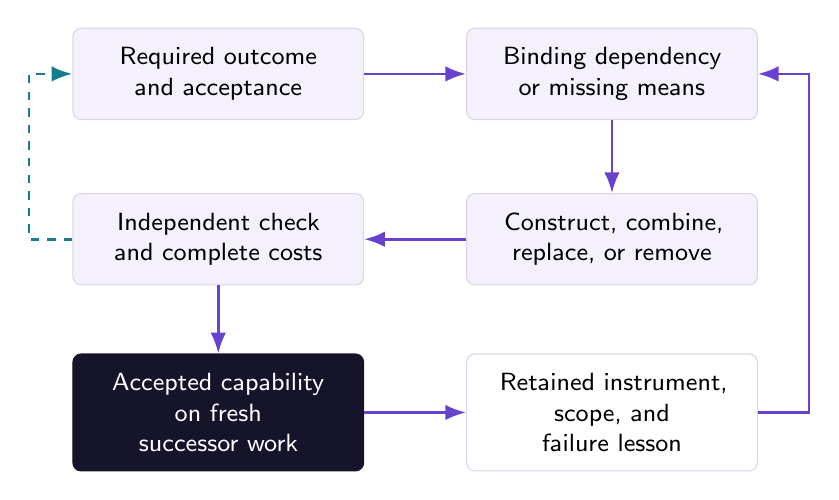
\begin{tikzpicture}[font=\small\sffamily,>=Latex,
 box/.style={draw=line,fill=wash,rounded corners=3pt,align=center,text width=3.2cm,minimum height=1.1cm,inner sep=7pt},
 arr/.style={->,draw=violet,line width=1pt}]
 \node[box] (purpose) at (0,0) {Required outcome\\and acceptance};
 \node[box] (constraint) at (5,0) {Binding dependency\\or missing means};
 \node[box] (construct) at (5,-2.1) {Construct, combine,\\replace, or remove};
 \node[box] (evidence) at (0,-2.1) {Independent check\\and complete costs};
 \node[box,fill=ink,text=white,draw=ink] (successor) at (0,-4.3) {Accepted capability\\on fresh\\successor work};
 \node[box,fill=white] (memory) at (5,-4.3) {Retained instrument,\\scope, and\\failure lesson};
 \draw[arr] (purpose)--(constraint);
 \draw[arr] (constraint)--(construct);
 \draw[arr] (construct)--(evidence);
 \draw[arr] (evidence)--(successor);
 \draw[arr] (successor)--(memory);
 \draw[arr] (memory.east) -- ++(.65,0) |- (constraint.east);
 \draw[arr,dashed,draw=teal] (evidence.west) -- ++(-.55,0) |- (purpose.west);
\end{tikzpicture}
\caption{The proposed loop changes the means of progress while keeping the authorized outcome visible.
The dashed return can expose an inadequate assessment instrument; changing the purpose requires a new contract.
The right-hand return is a hypothesis of useful inheritance, established only by a fresh comparison.
This is an architectural proposal, not a record of an executed autonomous discovery campaign.}
\label{fig:loop}
\end{figure}

\subsection{A repertoire of constructive moves}
\textbf{Create a discriminating observation.}
When available evidence cannot distinguish competing explanations, more inference on the same evidence can leave the uncertainty unchanged.
An intervention, sensor, reference standard, or new data source may change the information available.
Its calibration, acquisition rights, and failure modes are part of the construction.

\textbf{Construct a better representation.}
A representation can expose a conserved quantity, separate a nuisance variable, or turn a difficult search into a tractable one.
The retained abstraction must preserve distinctions that matter for the outcome.
Relational transfer supplies a disciplined source of proposals: analogy maps relationships across domains, while target-domain validity still requires a test \citep{gentner1983,gickholyoak1980}.

\textbf{Make production easier to verify.}
Evidence can be produced along with the result.
Traceable dependencies, certificates, and calibrated interfaces can reduce repeated checking under explicit scope conditions.
The gain depends on the cost of producing the evidence and on whether the checker remains sound for the new task.
The illustrative experiment in Section~\ref{sec:example} isolates this complementarity.

\textbf{Compose missing complements.}
An instrument without a usable protocol, or a protocol without an instrument, can be worthless.
A search that admits only individually improving edits can reject a useful pair.
Joint construction is legitimate when the combined costs and interface assumptions are evaluated.
It is not permission for an unlimited search through combinations.

\textbf{Reorganize voluntary cooperation.}
A useful outcome may be blocked by incompatible commitments, unverifiable delivery, financing timing, or the allocation of risk.
A changed arrangement can make existing technical capabilities usable.
Participation, outside options, enforceability, and actual funds need their own evidence \citep{boucher2026economy}.

\textbf{Remove recurring work.}
Standardization, validated invariants, direct delivery, or a better interface may eliminate an intermediate task.
The strongest accelerator may be the construction that makes a class of formerly necessary work unnecessary.
It must preserve material outputs, reliability, rights, and future obligations.

\subsection{Criticism can specify the next instrument}
A useful critic identifies a consequential discrepancy, supplies checkable support, and proposes a test that could settle it.
If the discrepancy is real, it can become a construction target: a missing observation, calibration, interface, or representation.
The critic's contribution is the actionable uncertainty it exposes.
An adjudicator should also be able to conclude that a criticism is unsupported.

Research on trained LLM critics supports the usefulness of assisted error detection while also documenting hallucinated criticisms \citep{mcaleese2024critics}.
Agreement among several model outputs is consequently an insufficient substitute for evidence.
Independence must be considered at the level of sources, measurements, implementations, and failure mechanisms, not merely the names assigned to agents.

\subsection{The architecture remains revisable}
The OUT research sequence supplies relevant mechanisms: observation in OUT-LEARN, representation in OUT-THINK, construction in OUT-DESIGN, arrangements in OUT-STRATEGISE, accepted execution in OUT-EXECUTE, and inherited means in OUT-EVOLVE \citep{boucher2026outseries}.
These mechanisms need not be invoked in that order or by separate agents.
\oa{} evaluates their contribution to the complete path and to subsequent work.
A simple procedure that preserves the outcome and wins the comparison should remain available.

\section{A finite-horizon theory of acceleration}\label{sec:model}

\subsection{A bottleneck model with an exact answer}
Suppose $n\ge1$ outputs each require a construction stage of duration $d>0$ and a verification stage of duration $v>0$.
There is one independent server per stage, an unlimited intermediate queue, no failures, and no other resource constraint.
All inputs are available at batch start.
Both stages process outputs in the same order and work whenever an eligible output is available.
Stages can overlap across outputs.
The accepted outputs and their quality requirements are fixed.
An acquisition period $K\ge0$ precedes the batch and cannot overlap it.

\begin{proposition}[Exact complete-batch time]\label{prop:pipeline}
Under these assumptions, the completion time is
\begin{equation}\label{eq:pipeline}
 T(n;d,v,K)=K+d+v+(n-1)\max(d,v).
\end{equation}
The total worker-time consumed is $W=K+n(d+v)$ when setup uses one worker.
\end{proposition}
\begin{proof}
After setup, construction finishes output $i$ at $id$.
Let $b_0=0$ and $b_i=\max(id,b_{i-1})+v$ be its verification completion time relative to the end of setup.
Induction gives $b_i=d+v+(i-1)\max(d,v)$.
Add $K$.
Summing the two servers' busy durations gives $n(d+v)$; overlap reduces elapsed time but does not erase resource consumption.
\end{proof}

If verification is the bottleneck, so that $v\ge d$, a construction speedup $s\ge1$ gives
\begin{equation}\label{eq:local}
 T_{\rm local}(n)=d/s+nv.
\end{equation}
Compared with the original $d+nv$, the saving is $d-d/s$ for the \emph{entire} batch.
The asymptotic interval between accepted outputs remains $v$.
This is a pipeline instance of the bottleneck logic associated with Amdahl's analysis \citep{amdahl1967}.
The formula is useful precisely because it exposes what a component benchmark leaves unchanged.

\subsection{Constructing a complementary accelerator}
Now add a trace-producing component with per-output overhead $\delta\ge0$ and a checker that reduces verification to $c>0$ when the trace and task scope are valid.
Either component alone leaves the original verification requirement in place.
Let the combined acquisition cost be $K$.
If $c\le d/s+\delta<v$, then
\begin{equation}\label{eq:bundle}
 T_{\rm bundle}(n)=K+c+n(d/s+\delta).
\end{equation}
The bottleneck has moved from verification to construction with evidence.

\begin{proposition}[When acquisition repays its delay]\label{prop:breakeven}
Under the conditions above, the bundle beats the local construction speedup exactly when
\begin{equation}\label{eq:breakeven}
 n\bigl(v-d/s-\delta\bigr)>K+c-d/s.
\end{equation}
Equality is a tie. If the conditions on stage ordering fail, compare the general formula in Equation~\eqref{eq:pipeline}.
\end{proposition}
\begin{proof}
Subtract Equation~\eqref{eq:bundle} from Equation~\eqref{eq:local}.
Strict positivity of the resulting expression is equivalent to Equation~\eqref{eq:breakeven}.
\end{proof}

The result has three practical implications.
First, acceleration depends on the workload horizon.
Second, the cost of producing evidence can consume the saving from checking it.
Third, removing one bottleneck can reveal another, so continued improvement requires a new diagnosis.
No term guarantees that the useful components can be discovered, built, or trusted in a real setting.

\subsection{Complementarity can defeat isolated improvement}
Let $T_{\varnothing}$ be the baseline, $T_P$ the trace producer alone, $T_V$ the checker alone, and $T_{PV}$ their combination.
It is possible that
\begin{equation}
 T_P>T_{\varnothing},\qquad T_V>T_{\varnothing},\qquad
 T_{PV}<T_{\varnothing}.
\end{equation}
This need not reflect mysterious synergy.
The checker requires a compatible trace; without it, its acquisition adds delay while verification falls back to the original route.
The trace alone adds work without reducing checking.
Compatibility is therefore a property to construct and test.

The broader importance of complementary inputs has established economic precedents \citep{kremer1993}.
Here the claim is narrower: a bounded search over a justified pair can be necessary even when each isolated edit loses.
A comparison should also permit an ordinary engineer or unrestricted conventional planner to make that same pair.

\section{An exact, reproducible worked example}\label{sec:example}

\subsection{What is supplied and what is executed}
The companion uses exact integer outputs and rational scheduling arithmetic.
The primary batch contains 12 inputs $x=1,\ldots,12$ and the subsequent batch contains 10 different inputs $x=101,\ldots,110$.
Both require the exact output $3x+7$.
An affine certificate names its domain, input, and coefficients; the checker verifies that the certificate matches the task and output.
A separate full checker remains available.
The program also corrupts products and attempts a transfer to a quadratic task to check rejection.

These tiny arithmetic tasks are \emph{carriers for an acceptance contract}.
The two checkers are simple computations, not implementations whose measured runtime differs by the large factors below.
All stage durations, acquisition costs, and scope conditions are author-supplied model inputs.
The experiment executes schedules and checks the stipulated model; it does not measure a real verification speedup or discover the certificate mechanism.
The subsequent inputs are public and prespecified, not concealed confirmation data.

\begin{table}[t]
\centering\small
\begin{tabularx}{\linewidth}{Yrr}
\toprule
Supplied parameter & Primary batch & Subsequent batch\\
\midrule
Outputs $n$ & 12 & 10\\
Construction duration $d$ & 4 & 8\\
Full verification duration $v$ & 12 & 20\\
Available construction speedup $s$ & 4 & 4\\
Trace overhead $\delta$ per output & 1 & 1\\
Certificate verification duration $c$ & 1 & 2\\
Combined construction/qualification $K$ & 24 & ---\\
Adaptation and requalification for reuse & --- & 8\\
\bottomrule
\end{tabularx}
\caption{Declared abstract time units. The fourfold construction engine is available to every policy with zero additional acquisition cost in this model. The primary bundle costs 4 for search, 6 each for the two components, 4 for integration, and 4 for qualification. Rebuilding on the subsequent batch pays 24 again plus 8 for adaptation and requalification.}
\label{tab:params}
\end{table}

\subsection{The comparison and its strongest control}
The two batches execute consecutively.
Each policy pays its own declared acquisition and transfer costs.
We compare the unchanged pipeline, faster construction, the isolated components, their combination, the combination with faster construction, and rebuilding the combination instead of retaining it.
The same outcome contract applies in every arm.

\begin{table}[t]
\centering\small
\begin{tabularx}{\linewidth}{Yrrrr}
\toprule
Declared workflow & Primary & Subsequent & Total time & Total work\\
\midrule
Original pipeline & 148 & 208 & 356 & 472\\
Faster construction & 145 & 202 & 347 & 376\\
Trace producer alone & 163 & 217 & 380 & 516\\
Checker alone & 162 & 216 & 378 & 494\\
Complementary bundle & 85 & 100 & 185 & 214\\
Bundle and faster construction & 49 & 40 & 89 & 118\\
Same bundle rebuilt for the subsequent batch & 49 & 64 & 113 & 142\\
\midrule
Ordinary reuse of the same supplied combination & 49 & 40 & 89 & 118\\
\bottomrule
\end{tabularx}
\caption{Exact executed model results. All workflows accept all 22 required outputs.
Time is elapsed model time; work sums busy time across servers.
The last row is an equal-content conventional workflow, not an additional discovery experiment.
Its tie is central to the interpretation. None of these numbers is measured AI performance, industrial throughput, or commercial profit.}
\label{tab:results}
\end{table}

The faster construction engine reduces total time from 356 to 347.
It does useful work, but the verification bottleneck absorbs most of its component-level advantage.
Either new component alone is worse than the original pipeline.
Their combination changes the bottleneck, and adding the equally available faster engine reduces the modeled total to 89.
The ratio $356/89=4$ is a property of this supplied instance, not an estimated acceleration factor for \oa{}.

Retaining the bundle saves 24 units relative to rebuilding it for the subsequent batch.
That difference is exactly the avoided reconstruction charge.
The full retained path still includes initial acquisition and subsequent adaptation.
An ordinary workflow with the same producer, checker, applicability rule, and costs achieves the same result.
The minimum among the seven declared policies is also 89; that finite comparison establishes neither global optimality nor cost-free discovery of the winning policy.

\begin{figure}[t]
\centering
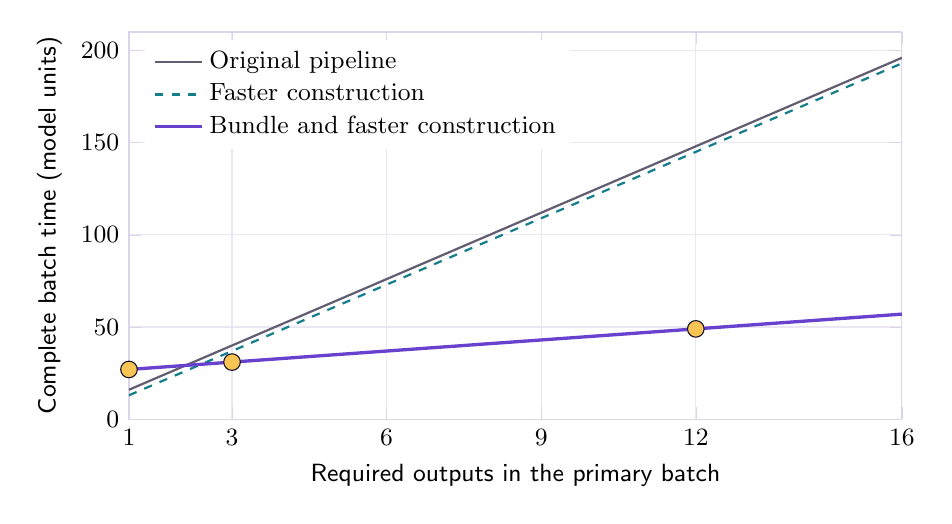
\begin{tikzpicture}
\begin{axis}[
 width=.94\linewidth,height=6.5cm,
 xlabel={Required outputs in the primary batch},
 ylabel={Complete batch time (model units)},
 xmin=1,xmax=16,ymin=0,ymax=210,
 xtick={1,3,6,9,12,16},ytick={0,50,100,150,200},
 axis line style={line},tick style={line},
 grid=major,grid style={line!60},
 legend style={at={(.02,.98)},anchor=north west,draw=none,fill=white,font=\small},
 label style={font=\small\sffamily},tick label style={font=\small},
 legend cell align=left]
 \addplot[muted,thick,domain=1:16,samples=16] {4+12*x};
 \addlegendentry{Original pipeline}
 \addplot[teal,thick,dashed,domain=1:16,samples=16] {1+12*x};
 \addlegendentry{Faster construction}
 \addplot[violet,very thick,domain=1:16,samples=16] {25+2*x};
 \addlegendentry{Bundle and faster construction}
 \addplot[only marks,mark=*,mark options={fill=gold,draw=ink},mark size=3pt] coordinates {(1,27) (3,31) (12,49)};
\end{axis}
\end{tikzpicture}
\caption{Construction can pay at one horizon and lose at another.
For this primary batch, $T_{\rm local}=1+12n$ and $T_{\rm bundle}=25+2n$.
The bundle wins for integer $n\ge3$ and loses for $n=1,2$.
Curves are exact model formulas, not empirical fits.}
\label{fig:horizon}
\end{figure}

\Needspace{9\baselineskip}
\subsection{When construction loses or transfer fails}
\textbf{Short horizon.}
For one output, the original pipeline takes 16 units, faster construction takes 13, and the complete bundle takes 27.
Building the accelerator is the wrong timing decision in this instance.

\Needspace{6\baselineskip}
\textbf{Invalid transfer.}
The affine certificate does not establish a quadratic outcome.
A forced use on $x^2+7$ rejects all four test outputs, while the full-verification fallback accepts the correct products.
Fast rejection is useful behavior, but it is not successful completion of the original job.
Its consumed time and work remain costs.

\Needspace{6\baselineskip}
\textbf{Corrupted evidence.}
Correct products must be accepted; altered values and incompatible certificate fields must be rejected.
A checksum or internally consistent trace cannot replace a semantic connection to the required outcome.
The checks in the companion are finite contract regressions, not a security proof of a general certification service.

\Needspace{6\baselineskip}
\textbf{Construction and retention are different interventions.}
The full advantage over the original pipeline combines faster production, a supplied verification effect, compatibility, acquisition, and retention.
The 24-unit retention comparison isolates only rebuilding versus reuse in the declared model.
Neither comparison identifies an improved discovery policy.

\subsection{What the illustration establishes}
The model establishes that local speed, complete-path time, component complementarity, and successor reuse can have different verdicts under one unchanged output contract.
It also gives an inspectable counterexample to the claim that building more reusable machinery is always faster.
The parameterization is intentionally transparent; no claim of representative frequencies, novel algorithms, or autonomous discovery follows.

The necessary next step is to replace stipulated effects with independently measured constructions on consequential tasks.
For that step, the evaluation design matters more than increasing the size of the arithmetic example.

\Needspace{10\baselineskip}
\section{From inherited equipment to a better inventor}\label{sec:inheritance}

\subsection{Three things a mission can leave behind}
A completed mission can leave an \emph{instrument} that performs useful work, an \emph{applicability model} that predicts when using it is warranted, and a \emph{constructor} that produces related instruments for new requirements.
Each is a different artifact.
An instrument can work while its routing rule fails.
A routing rule can be useful without generating new tools.
A constructor can produce many artifacts without improving useful discovery after verification costs.

Structural memory should retain the executable mechanism, supporting conditions, disconfirming cases, integration requirements, and cost.
It should distinguish an observed failure from an unknown cause.
The useful memory can be concise: retaining every transcript is neither necessary nor sufficient for transfer.
Compression becomes a claim to test when it can discard information needed by future work.

\subsection{A factorial test of discovery improvement}
Let $\pi_0,\pi_1$ be old and revised discovery procedures, and $\K_0,\K_1$ old and enriched starting capability sets.
Run fresh matched campaigns in all four conditions:
\begin{equation}
 \begin{aligned}
 Y_{00}&=Y(\pi_0,\K_0), &Y_{01}&=Y(\pi_0,\K_1),\\
 Y_{10}&=Y(\pi_1,\K_0), &Y_{11}&=Y(\pi_1,\K_1).
 \end{aligned}
\end{equation}
$Y$ can be accepted outcomes by a fixed resource endpoint, complete time to a matched outcome, or a preregistered utility under hard acceptance constraints.
The direction of improvement must match the metric.

\begin{table}[h]
\centering\small
\begin{tabularx}{\linewidth}{P{3.5cm}YY}
\toprule
 & Original assets $\K_0$ & Enriched assets $\K_1$\\
\midrule
Original discovery policy $\pi_0$ & Reference campaign $Y_{00}$ & Asset effect under the original policy $Y_{01}$\\
Revised discovery policy $\pi_1$ & Policy effect at original assets $Y_{10}$ & Combined result and interaction $Y_{11}$\\
\bottomrule
\end{tabularx}
\caption{Proposed campaign-level experiment. It has not been executed for this paper.
Asset and policy effects require matched resources, task distributions, information, and independent assessment.
The interaction may be beneficial, harmful, or absent.}
\label{tab:factorial}
\end{table}

For a higher-is-better scalar metric, $Y_{10}-Y_{00}$ and $Y_{11}-Y_{01}$ describe policy effects at fixed assets.
$Y_{01}-Y_{00}$ describes an asset effect under the original policy.
Replicated, properly assigned campaigns are needed to estimate these differences and their uncertainty.
Report effects conditional on supplied starting assets separately from programme-level effects that charge acquisition of those assets.
A difference-in-differences expression alone is not causal identification.
If only $Y_{11}>Y_{00}$ is observed, equipment, policy, and their interaction remain confounded.

Use equal-content ordinary reuse as an additional control.
If a conventional workflow given the same retained material achieves the same result, the evidence supports the material's usefulness, while a special discovery-method advantage remains unestablished.
The resulting evidence supports using the asset wherever its applicability and economics hold.

\subsection{Compounding has costs and floors}
A simple thought model clarifies the meaning of the infinity mark.
Suppose comparable mission $k$ takes
\begin{equation}\label{eq:floor}
 t_k=h+u_0\rho^k+a_k,\qquad
 h>0,\ u_0>0,\ 0<\rho<1,\ a_k\ge0,
\end{equation}
where $h$ is a persistent serial floor, $u_0\rho^k$ the part improved by inherited means, and $a_k$ the acquisition and adaptation delay.
For $m$ missions indexed from $k=0$,
\begin{equation}\label{eq:sumfloor}
 \sum_{k=0}^{m-1}t_k
 =mh+u_0\frac{1-\rho^m}{1-\rho}+\sum_{k=0}^{m-1}a_k
 \ \ge\ mh.
\end{equation}
Even geometrically improving one component does not complete infinitely many comparable missions in finite time when a positive floor remains.
Acquisition costs can also make individual generations slower.
The model assumes the improvement factor; it does not predict or prove its existence.

The frontier may change in other ways.
A new instrument can support harder outcomes without reducing elapsed time.
A new arrangement can lower deployment cost without making research faster.
These are valuable possibilities, but the labels should follow the measured outcome.
The infinity mark expresses continued revisability of the means, not an empirical claim of unbounded growth.

\section{An evaluation contract for consequential acceleration}\label{sec:evaluation}

\subsection{Freeze the comparison at the right boundary}
An experiment should state the outcome, target population, permitted actions, initial information, starting assets, horizon, cost model, candidate-selection rule, and stopping conditions before confirmation.
Freeze the candidate implementation before the fresh evaluation that supports its claim.
Exploration may remain adaptive; confirmation should not silently become another development set.
Adaptive reuse of evidence can overfit the evaluation process, motivating sealed confirmation or a justified adaptive-valid method \citep{dwork2015holdout}.

The finite experiment budget serves identification and resource accounting.
It is not a permanent ceiling on the business or an instruction to abandon a useful long-term mission.
The campaign can continue through registered extensions while preserving previous attempts, costs, and verdicts.

\subsection{Give strong alternatives the same opportunity}
\begin{table}[t]
\centering\small
\begin{tabularx}{\linewidth}{P{3.25cm}Y}
\toprule
Comparator & Alternative explanation it addresses\\
\midrule
Strong current workflow & The apparent gain comes from comparing against an avoidably weak incumbent.\\
More resources in the same formulation & The improvement comes from extra computation, labor, or time.\\
Unrestricted competent alternative & The construction is available to ordinary engineering with the same information and permissions.\\
Equal-content ordinary reuse & The retained asset helps, but the proposed discovery architecture adds no benefit.\\
Rebuild from the same starting resources & The claimed successor gain is only an uncharged inherited asset.\\
Component and applicability ablations & The proposed mechanism, its complement, or its scope rule is not causally responsible.\\
\bottomrule
\end{tabularx}
\caption{Controls are selected for the claim. An appropriate strong alternative can be simpler than the proposed system.
The experimental sweep and tuning consume resources and must not become an invisible advantage.}
\label{tab:controls}
\end{table}

Human productivity comparisons require a competent human workflow with conventional software retaining its genuine automation.
An AI workflow should count all actual human intervention and disclose whether it is autonomous or hybrid.
Human-plus-AI providers, other autonomous systems, and self-service are additional practical alternatives.
These groups answer different questions and should not be silently substituted for one another.
Research-engineering benchmarks such as RE-Bench illustrate why conclusions can depend on the task and resource horizon \citep{wijk2025rebench}.
This manuscript runs no such human comparison.

\subsection{Preserve the denominator}
Count all selected candidates, attempted transfers, failed experiments, refusals, and consumed resources.
If the claim concerns an entire discovery system, the unit of replication is the campaign, not each correlated output emitted by the same campaign.
Predeclare the primary comparison and treatment of repeated looks.
Use uncertainty estimates compatible with the actual sampling design.
The deterministic illustration requires no statistical confidence interval because it enumerates a specified model, not a sampled population.

A valid report gives at least acceptance, non-completion, elapsed time, total work, cash costs or modeled cost ranges, quality, residual obligations, and scope failures.
Do not aggregate these into a headline rate that hides a changed outcome or larger budget.
For a claim about improved discovery, include search and acquisition; for a deployment choice, also show the incremental decision using currently available assets.

\subsection{An evaluator can improve without approving itself}
The acceptance instrument may miss a consequential defect.
Discovering that gap can be a productive result.
A candidate may propose a stronger evaluator, but it cannot obtain a promotion merely by replacing its own judge.
Validate the revised instrument on separate evidence, preserve previous results under their original meaning, and rerun or relabel the affected comparison.
Changing the authorized outcome requires a newly stated task.

For scientific or physical work, distinguish model agreement from external measurement.
A simulator that shares the candidate's mistaken assumption can reward the same error.
Independent instruments, interventions, source checks, and out-of-scope challenges should be chosen according to the failure being tested.
More critics alone do not establish this independence.

\subsection{A compact promotion rule}
Promote a reusable capability only when its proposed use has valid acceptance evidence, a relevant gain under the declared comparison, and acceptable lifecycle costs and obligations.
Retain the incumbent when the comparison favors it.
Retain an informative failure lesson when the proposed capability loses.
Promote a new discovery procedure only after the stronger campaign-level evaluation.

This rule concerns claims and adoption decisions, not a requirement to invent a novel proof for every ordinary operation.
Established engineering can be used with normal applicability and correctness checks.
New scientific or recursive-improvement claims require the additional evidence appropriate to their scope.

\section{From faster capability to funded expansion}\label{sec:economics}

\subsection{Invent the complete productive arrangement}
A technically useful instrument can remain economically inaccessible.
The complete arrangement includes the valuable outcome, the producer, the evidence required for acceptance, the rights to act, the willing participants, and the timing of funds.
These elements should be searched jointly when any of them blocks viability.
This extends the construction emphasis of \citet{boucher2026economy,boucher2026frontier}.

Consider, as a proposed research direction, a service that reconstructs a historical measurement series for a question no one explicitly measured at the time.
The opportunity exists only where recorded evidence contains enough information.
The construction might combine heterogeneous archives, a defensible measurement model, uncertainty calibration, and acceptance of the resulting product.
If observational equivalence prevents identification, additional verbal reasoning cannot manufacture the missing facts.
The useful outcome may instead be a bounded estimate or a documented non-identifiability result, if that is what the beneficiary actually needs.
An altered deliverable requires explicit acceptance.

The commercially significant invention could be the instrument, the arrangement for commissioning it, or their combination.
The existence of a large possible market is not evidence that a buyer accepts the deliverable, pays the price, or funds the supplier's obligations.
These are separate empirical questions.

\subsection{Separate knowledge, capability, profit, and available funds}
Knowledge can improve without an installed productive capability.
A capability can improve without a profitable sale.
A profitable sale can repeat while the capability remains unchanged.
An accounting profit can coexist with inadequate cash for the next investment.
Each link in a claimed expansion sequence requires its own receipt.

Write a declared period's profit schematically as recognized revenue minus complete attributable expenses under a stated accounting convention.
Let $C_{\rm unrestricted}(t)$ be cash on hand that is available for the modeled purpose, including opening funds and received financing under their actual terms.
Write funds available for a new commitment separately as
\begin{equation}
 C_{\rm available}(t)=C_{\rm unrestricted}(t)-R_{\rm unpaid}(t),
\end{equation}
where $R_{\rm unpaid}$ covers unpaid obligations and protected reserves not already deducted or restricted out of the cash term.
Count each obligation once; cash already paid is already absent from cash on hand.
Forecast sales, unsigned financing, and uncollected invoices cannot be substituted for current spendable funds.
The expression is a planning distinction, not a replacement for an actual financial ledger or applicable accounting rules.

\textbf{Profit without investable cash.}
In an illustrative accrual account measured in thousands of dollars, initial cash is 20.
Accepted invoiced revenue is 20 but remains uncollected.
Expenses total 12, of which 8 have been paid and 4 remain payable.
Profit is 8, gross cash is 12, and cash after reserving the payable is 8.
A new investment requiring 10 is deferred.
Deferral does not erase the positive profit result; the positive profit does not finance the unavailable cash.
This is an arithmetic example, not an observed transaction or a claim of a fully costed business.

\subsection{Cooperation and optimality have explicit conditions}
A proposed voluntary arrangement should make each required participant's expected outcome acceptable relative to their outside option under a stated information and risk model.
For participant $j$, a minimal modeled condition is
\begin{equation}
 \mathbb E[U_j\mid \text{arrangement, information}]
 \ge U_j^{\rm outside}.
\end{equation}
This inequality does not establish consent, enforceability, truthful reporting, incentive compatibility, or equilibrium.
Those require their own mechanisms and assumptions.
Rivals may copy the capability, prices may change, and beneficiaries may choose not to purchase.

An optimality claim must specify the feasible actions, information, objective, funding, and response model.
A finite optimizer can establish an optimum inside its supplied problem; it cannot certify the globally best enterprise.
The scheduling example's ordinary tie is an intentionally visible instance of this boundary.

\subsection{Three different successor relationships}
An earlier mission \emph{finances} a later mission when traceable available funds pay its costs.
It \emph{enables} that mission when an earlier asset changes the later mission's feasibility or performance under a matched counterfactual.
A mission can also simply occur later.
Chronology alone establishes neither financing nor enablement.

To claim a connected commercial flywheel, demonstrate accepted delivery, complete costs, settlement, protected obligations, the actual reinvestment decision, and the successor outcome.
To claim discovery acceleration as well, add the policy-and-assets comparison.
The repository's US\$3 billion trailing-365-day profit milestone is a separate, unachieved project objective; the model results here do not contribute dollars toward it.
Starting capital and financing must be stated in any relevant campaign rather than inferred from the paper.

\section{Relationship to prior research}\label{sec:related}

\textbf{Knowledge and complementary production.}
Endogenous growth theory makes investment in knowledge part of the economic model \citep{romer1990}.
Recombinant growth studies the production of ideas through recombination and the burden of turning possibilities into usable knowledge \citep{weitzman1998}.
Complementarity and the increasing burden of knowledge motivate attention to the full productive arrangement and the costs of learning \citep{kremer1993,jones2009}.
\oa{} does not infer a macroeconomic growth rate from these foundations.
It proposes inspectable mission-level constructions and comparisons.

\textbf{Exploration and constructive search.}
The allocation between using known capabilities and exploring new ones is longstanding \citep{march1991}.
Structural analogy supplies a mechanism for candidate generation \citep{gentner1983,gickholyoak1980}.
Enhanced POET demonstrates the co-generation of challenges and solutions in an open-ended reinforcement-learning setting \citep{wang2020poet}.
These precedents rule out treating open-endedness, transfer, or the search for new tasks as new ideas originating here.

\textbf{AI-assisted scientific and algorithmic discovery.}
AlphaTensor studies algorithm discovery for matrix multiplication \citep{fawzi2022}.
FunSearch searches programs using an evaluator \citep{romeraparedes2024}.
AlphaEvolve extends evaluator-driven code improvement and reports benefits to computational infrastructure, including components supporting the model used by the system \citep{novikov2025alphaevolve}.
It is therefore already a direct precedent for improving means that support further AI work.
The present paper does not claim to be the first recursive accelerator or automated inventor.

Physical research also depends on constructed instruments and execution systems.
The mobile robotic chemist of \citet{burger2020} is a concrete example of autonomous experimental search through laboratory work.
Such systems motivate the measurement-and-deployment boundary; an executable software demonstration does not reproduce their physical validation.

\textbf{Verification and evaluation.}
Trained critics can help identify errors but can introduce erroneous criticism \citep{mcaleese2024critics}.
Adaptive data analysis makes the reuse of evaluation evidence a methodological concern \citep{dwork2015holdout}.
RE-Bench provides a concrete approach to comparing AI research engineering with expert effort under explicit budgets \citep{wijk2025rebench}.
Our proposed evaluation combines these concerns with inherited assets, component interactions, and full acquisition costs.

\textbf{The specific synthesis.}
The Transformational Intelligence programme makes the problem-solving setup revisable while preserving the intended purpose \citep{boucher2026ti}.
Related work considers reusable experimental interfaces and purpose-preserving removal of unnecessary subproblems \citep{boucher2026world,boucher2026original}.
The companion AGI ALPHA FLYWHEEL paper connects retained knowledge, productive capability, and earned capital to a better starting point for subsequent work \citep{boucher2026flywheel}.
\oa{} makes the temporal consequence explicit: which construction changes the path to the next accepted outcome, when does that construction repay its burden, and when does inheritance improve the process that finds further constructions?
That is a proposed research contract, not evidence that a general system already satisfies it.

\section{A programme for making new activities possible}\label{sec:programme}

\subsection{Select for consequence, then construct a decisive test}
Begin with a valuable outcome whose current route is inaccessible or uneconomic under credible assumptions.
Compare materially different complete arrangements, including replacing the service or method.
Identify the uncertainty whose resolution could change a construction or investment decision.
Then build the smallest instrument or arrangement that can decisively test it.
The test can be small even when the consequence of success is large.

Three directions illustrate the search space:
\begin{enumerate}
 \item \textbf{Question-defined measurement.}
 Construct a defensible new measurement from available evidence, with an explicit identifiability boundary, and test whether an independent user can use it for the intended decision.
 The first decisive test is source-grounded measurement validity.
 \item \textbf{Reusable experimental infrastructure.}
 Construct a fixture, calibration method, or simulation-to-measurement bridge that reduces the complete cost of testing a new design family.
 The first decisive test is a changed subsequent design whose acceptance survives independent measurement.
 \item \textbf{Verifiable autonomous delivery.}
 Construct a production process and voluntary acceptance arrangement that make a previously uneconomic service deliverable.
 The first decisive test includes the actual deliverable, acceptance, full cost, and timing of funds.
\end{enumerate}
These are proposed classes of opportunity, not demonstrated businesses.
They should compete against simpler complete alternatives.
None is permanently privileged by the framework.

\subsection{Five falsifiable hypotheses}
\textbf{H1: Complete-path targeting.}
Under matched budgets, choosing interventions by their effect on time to accepted outcome outperforms choosing them by local generation throughput on tasks with multiple bottlenecks.
This fails if the gain disappears under competent end-to-end controls.

\textbf{H2: Constructive criticism.}
Turning verified discrepancies into targeted instrument-construction proposals improves the rate of accepted useful discoveries after criticism and adjudication costs.
This fails if additional checking consumes the saving or produces no better constructions.

\textbf{H3: Complementary construction.}
A bounded, interface-aware search over combinations opens useful outcomes missed by an equally funded sequence of isolated improvements.
This fails if the equally funded isolated-improvement control matches or exceeds the combination search.
Superiority to unrestricted ordinary search is a separate comparison.

\textbf{H4: Generative inheritance.}
With retained material and resources held fixed, a revised discovery policy using qualified constructors and applicability knowledge improves fresh instrument-building campaigns over an ordinary workflow.
This fails if the prespecified policy effect at fixed assets is absent; an asset-only gain does not establish improved discovery.

\textbf{H5: Economic continuation.}
A verified capability can support accepted, profitable delivery and an actually funded successor under voluntary participation.
This fails commercially if demand, collection, full costs, or obligations prevent funded continuation, even when the technical construction works.

Each hypothesis requires an outcome population, budget, comparison, and stopping rule.
No single favorable case establishes all five.

\subsection{Limits of the present contribution}
The worked example is supplied, small, and deterministic.
Its timing parameters are not calibrated from industrial measurements.
The certificate does not establish the validity of arbitrary scientific claims.
The conventional tie prevents a claim of method superiority.
The proposed factorial campaigns, human comparisons, real-market deployments, and physical experiments remain unexecuted here.

Persistent acceleration could fail because discoveries become harder, complements are scarce, verification grows more expensive, inherited assumptions become obsolete, or funding arrives too late.
An economically successful system may also rationally repeat a known service instead of investing in invention.
The framework needs to recognize those outcomes without treating continued research as an obligatory ritual.

\section{Conclusion}
Progress depends on a production process: information must become a construction, a construction must survive evaluation, and a useful capability must become usable in the next setting.
Intelligence can act on that process itself.
It can create a missing instrument, expose a better representation, build a complementary interface, or remove a dependency that belonged only to the old method.

\oa{} gives this ambition a comparative meaning.
Measure complete time to accepted outcomes, charge the construction of the advantage, test reuse on subsequent work, and distinguish improved equipment from improved discovery.
When commerce is part of the claim, verify the voluntary exchange and the funds that actually support continuation.

The exact illustration makes the interpretation concrete: local speed can leave the bottleneck intact; complementary construction can pay; a short horizon can reverse the choice; an invalid transfer must fail; and ordinary reuse can match the proposed combination.
Those boundaries make the larger research question testable.

\principle{The next important advance may be a better way to reach the advance after it.}

\appendix
\section{Derivations and reporting details}\label{app:derivations}

\subsection{The two-stage recurrence}
For $d\ge v$, each verification finishes no later than the next construction completes:
$b_i=id+v$.
For $v\ge d$, the verifier remains busy after the first output:
$b_i=d+iv$.
Both cases equal $d+v+(i-1)\max(d,v)$.
The proof assumes homogeneous stage durations within each batch.
Heterogeneous tasks, shared machines, failures, finite buffers, and changing priorities require a corresponding scheduling model.
Equation~\eqref{eq:pipeline} should not be transplanted to such a setting without checking its assumptions.

\subsection{A general pairwise break-even test}
For two designs $(d_0,v_0,K_0)$ and $(d_1,v_1,K_1)$, write
$m_j=\max(d_j,v_j)$.
The candidate is faster exactly when
\begin{equation}
 (n-1)(m_0-m_1)>
 (K_1-K_0)+(d_1+v_1)-(d_0+v_0).
\end{equation}
If the steady-state intervals tie, only setup and pipeline fill differ.
If the candidate has a worse interval, increasing the workload can reverse an early advantage.
This is a conditional comparison of given designs, not an algorithm for discovering the best design.

For the primary example with a faster constructor, the original local path is $1+12n$ and the complete bundle is $25+2n$.
The strict advantage condition is $10n>24$, hence $n\ge3$ for integer batch sizes.
For the subsequent batch with reuse, the local path is $2+20n$ and the bundle is $10+3n$.
The changed workload pays its separate adaptation cost of 8.
The two batches are serial, so their completion times add; their constituent servers overlap only within a batch.

\subsection{Resource accounting}
For the winning supplied combination, primary work is
$24+12(2+1)=60$.
Subsequent work is $8+10(3+2)=58$.
Total work is 118, whereas total elapsed time is $49+40=89$.
Those quantities answer different questions.
Neither is a monetary price, energy estimate, measured model-token count, or human-labor estimate.

The public experiment's comparison sweep is research overhead.
It does not grant a deploying policy free access to an empirically discovered winner.
The companion reports the declared arms and their complete modeled paths.
Any real search procedure selecting among such arms must include its selection and failed-attempt costs in a discovery claim.

\section{Reproduce and inspect the research artifact}\label{app:reproduce}
The companion directory is
\href{\repo/tree/main/docs/research/out-accelerate}{\texttt{docs/research/out-accelerate}}.
It contains a standard-library Python program, the frozen output table, compact results, a review note, and build instructions.
No model API, credentials, external dataset, or paid service is needed to reproduce the analytical example.

\begin{lstlisting}
python3 docs/research/out-accelerate/acceleration_witness.py \
  --output-dir /tmp/out-accelerate-replay
\end{lstlisting}

The program uses exact rational arithmetic, validates the pipeline recurrence, checks the displayed totals, preserves component losses and short-horizon loss, verifies correct outputs, and rejects corrupted or out-of-scope certificates.
The public inputs and executable checks make the illustration inspectable.
They do not create an independent empirical benchmark simply by being reproducible.

Compile the paper from \texttt{docs/research} with a TeX distribution containing XeLaTeX, \texttt{latexmk}, BibTeX, and DejaVu Sans Mono.
The source prefers TeX Gyre Pagella and Heros, then the compatible URW OpenType fonts on Linux, with Latin Modern fallbacks:
\begin{lstlisting}
latexmk -xelatex -interaction=nonstopmode \
  -halt-on-error -no-shell-escape out-accelerate.tex
\end{lstlisting}
The diagrams and model curves are vector graphics generated by the LaTeX source.
The bibliography is supplied separately.
Build products other than the final PDF need not be committed.

\textbf{Authorship and assistance.}
The manuscript was prepared with AI-assisted research, coding, and editorial review.
The experiment is an authored model with supplied mechanisms.
Neither the author line nor the review process implies that an autonomous system discovered those mechanisms.
The contribution and evidence status are as stated in the abstract.

\section{A reusable campaign specification}\label{app:contract}
A concise prospective record should answer the following questions in concrete terms.
It need not impose a new framework on work that already has adequate records.
\begin{enumerate}
 \item \textbf{Outcome.} What valuable result is required, for which population, and what must remain unchanged?
 \item \textbf{Constraint.} Which dependency or missing means blocks the current complete route? What evidence would show that diagnosis is wrong?
 \item \textbf{Construction.} What will actually be built, replaced, combined, or removed? What are its interfaces and scope conditions?
 \item \textbf{Alternative.} What is the strongest complete conventional route with the same permissions, information, and resources?
 \item \textbf{Accounting.} Where does the clock begin? Which costs, failed attempts, acquired assets, and obligations are charged?
 \item \textbf{Confirmation.} What is frozen, what remains adaptive, how is final acceptance assessed, and what stops this experiment?
 \item \textbf{Successor.} Which fresh task tests inheritance, and what ablation distinguishes retained capability from extra resources or saved answers?
 \item \textbf{Discovery.} Is a better inventor claimed? If so, where are the policy-by-assets campaigns and equal-content controls?
 \item \textbf{Economics.} If commercial expansion is claimed, where are voluntary acceptance, settlement, complete costs, and spendable funding?
 \item \textbf{Decision.} What passed, failed, or remains unknown; which claim is warranted; and what is the next useful action?
\end{enumerate}
The experiment can produce a successful construction, a useful negative result, or a reason to stop.
Its purpose is to change what can be credibly done next.

\clearpage
\bibliographystyle{plainnat}
\bibliography{out-accelerate}
\end{document}
